\clearpage
%%=========================================
%\section[Surface Analysis of Substrate B with Surface Pre-Growth Preparation]{Surface Analysis of Substrate B with Surface Pre-Growth Preparation%
%   \sectionmark{Surface Analysis of Pre-Growth Substrate B}}\sectionmark{Surface Analysis of Pre-Growth Substrate B}\label{sec:subBb}
   
\section{Surface Analysis of Substrate B after fine Polishing and Etching}

As substrate B was roughly polished by the vendor, the surface pre-growth preparation consisted of both polish and a \ce{Br}:methanol etch. The dark field images taken of the surface of substrate B after polishing and etching showed that the surface pre-growth preparation had improved the surface considerably, compare Fig.~\ref{fig:subBa_om_df} and Fig.~\ref{fig:subBb_om_df}. The previously observed deep surface scratches were removed and there were far less particles and other features on the substrate surface. In comparison to substrate B, substrate B2 had more particles larger than \SI{0.5}{\micro\metre} on the surface, but it too was without deep surface scratches and large features, see Fig.~\ref{fig:subB2b_om_df}.

\begin{figure}[htbp]
    \centering
    \mySubfigure{0.8\linewidth}{subBb_om_n016.jpg}[fig:subBb_om_df]
    \par\bigskip
    \mySubfigure{0.8\linewidth}{subB2b_om_5x_n022.jpg}[fig:subB2b_om_df]
    \caption[Dark field optical microscopy image of substrate B and B2 with surface pre-growth preparation.]{Dark field optical microscopy image of \subref{fig:subBb_om_df} the upper left corner of substrate B with surface pre-growth preparation and \subref{fig:subB2b_om_df} the centre of substrate B2 with surface pre-growth preparation.}\label{fig:subBb_and_subB2b_om_df}
\end{figure}

\Ac{sem} shows the surface at a higher magnification and revealed that there were smaller particles distributed over the surface as well. A typical area in the centre of substrate B and substrate B2 can be seen in Fig.~\ref{fig:subBb_sem_typical_centre} and Fig.~\ref{fig:subB2b_sem_typical_centre} respectively. The particle density in the two images were \SI{2e+08}{\centi\metre^{-2}} and \SI{6e+07}{\centi\metre^{-2}} respectively. The particles on both substrates had lengths of \SIrange{20}{50}{\nano\metre}. 

\begin{figure}[htbp]
    \mySubfigure{0.49\textwidth}{subBb_sem_05a_m014.png}[fig:subBb_sem_typical_centre]
    \hfill
    \mySubfigure{0.49\textwidth}{subB2b_sem_02b_m004.png}[fig:subB2b_sem_typical_centre]
    \caption[\Ac{sem} images of typical areas on substrate B and B2 with surface pre-growth preparation.]{\Ac{sem} images of a typical area near the centre of \subref{fig:subBb_sem_typical_centre} substrate B and \subref{fig:subB2b_sem_typical_centre} substrate B2 after surface pre-growth preparation.}\label{fig:subBb_and_subB2b_sem_typical}
\end{figure}

%%=========================================
% Twin boundaries.
Four twin boundaries were visible to the naked eye after polish and etch. Two in the upper left corner and two that spanned from the lower right corner to the middle of the upper edge, see Fig.~\ref{fig:subBb_twins_illustration}. By doing an Everson etch it was established that the area between the lines in the upper left corner and between the two other lines were (111)B-oriented, while the surrounding area were twins \citep{everson1995etch}. A part of the twin boundary near the upper left corner can be seen in Fig.~\ref{fig:subBb_sem_twins}. It formed a piecewise straight line with steps that change the direction by \SI{\pm 45}{\degree} every \SIrange{10}{200}{\micro\metre}.

\citet{ashida2015crystallographic} studied the dependence of \ac{sem} contrast on crystallographic orientation in \ce{SiC} polytypes. They found that features looked brighter when the direction of the incident electron beam was almost parallel to the topmost stacking sequence direction. However, the formation mechanism of the \ac{sem} contrast is still under discussion. This could explain why there was a visible contrast in \ac{sem} at the twin boundaries.

\begin{figure}[htbp]
    \centering
    \begin{subfigure}[t]{0.4\linewidth}
        \caption{}\label{fig:subBb_twins_illustration}
        \centering
        \begin{tikzpicture}[remember picture]
          \node[anchor=south west,inner sep=0] (imageA) {
\includegraphics[width=\linewidth]{subBb_twins.png}};
          \begin{scope}[x={(imageA.south west)},y={(imageA.north east)}]
            \node[coordinate] (A) at (0.033\linewidth, 0.967\linewidth) {};
          \end{scope}
        \end{tikzpicture}
    \end{subfigure}
    \hfill
    \begin{subfigure}[t]{0.5333\linewidth}
        \caption{}\label{fig:subBb_sem_twins}
        \centering
        \begin{tikzpicture}[remember picture]
          \node[anchor=south west,inner sep=0] (imageB) {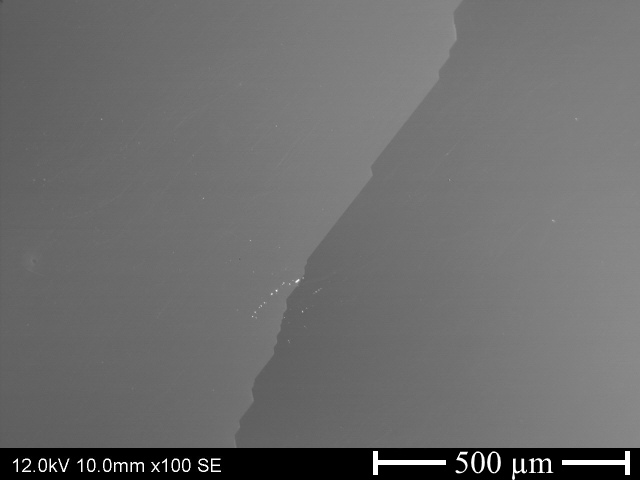
\includegraphics[width=\linewidth]{subBb_sem_01_m005.png}};
          \begin{scope}[x={(imageB.south west)},y={(imageB.north east)}]
            \node[coordinate] (B) at (0.5,0.5) {};
          \end{scope}
        \end{tikzpicture}
    \end{subfigure}
    \caption[Twin boundaries on substrate B.]{\subref{fig:subBb_twins_illustration} Illustration of the location of twin boundaries on substrate B and \subref{fig:subBb_sem_twins} \iac{sem} image of the twin boundary near the upper left corner.}\label{fig:subBb_twin_boundaries}
    % Draw arrow.
    \begin{tikzpicture}[remember picture,overlay]
      \draw[->, red, line width=0.5mm ] (B) -- (A);
    \end{tikzpicture}
\end{figure}

%%=========================================
\subsection{Particles}

Four different types of particles were observed on the surface of substrate B and substrate B2 after surface pre-growth preparation, see Fig.~\ref{fig:subBb_sem_w_eds}. They will be described and identified in the following.

\begin{figure}[htbp]
    \centering
    \begin{subfigure}[t]{\textwidth}
        \caption{}\label{fig:subB2b_alumina}
          \begin{minipage}[c]{0.43\linewidth}
            \centering
            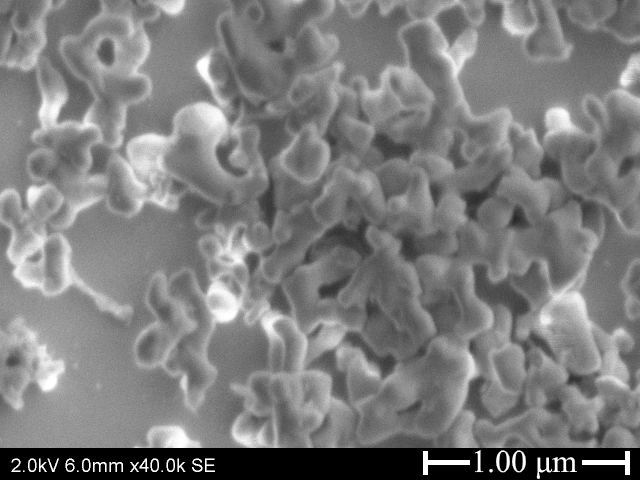
\includegraphics[width=\linewidth]{subB2b_sem_03_m006.png}
          \end{minipage}
          \hfill
          \begin{minipage}[c]{0.43\linewidth}
            \centering
            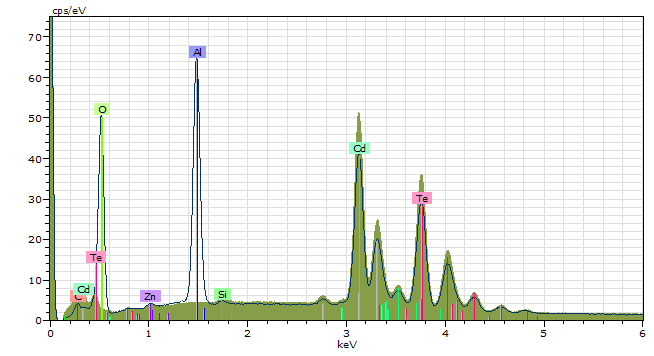
\includegraphics[width=\linewidth]{subB2b_sem_03_m006_eds.png}
          \end{minipage}
          \begin{minipage}[c]{0.11\linewidth}
            \centering
            \atomicTable[\ce{O}&\SI{43.0}{}][\ce{Al}&\SI{24.7}{}][\ce{Cd}&\SI{15.2}{}][\ce{Te}&\SI{14.8}{}][\ce{C}&\SI{1.6}{}][\ce{Zn}&\SI{0.5}{}][\ce{Si}&\SI{0.2}{}]%OK
          \end{minipage}
    \end{subfigure}
    \par\bigskip
    \begin{subfigure}[t]{\textwidth}
        \caption{}\label{fig:subB2b_czt}
          \begin{minipage}[c]{0.43\linewidth}
            \centering
            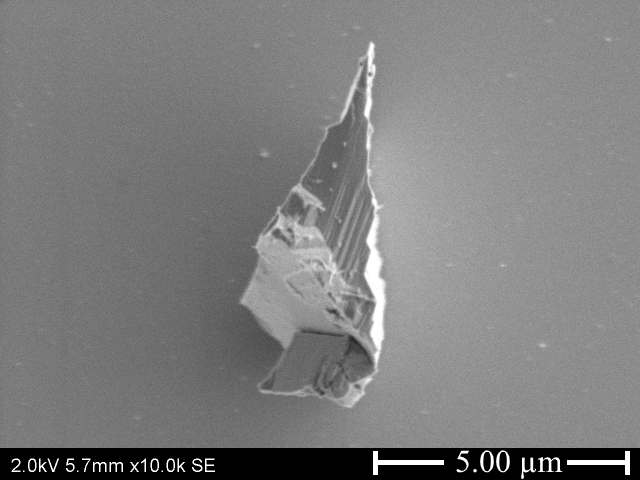
\includegraphics[width=\linewidth]{subB2b_sem_03_m002.png}
          \end{minipage}
          \hfill
          \begin{minipage}[c]{0.43\linewidth}
            \centering
            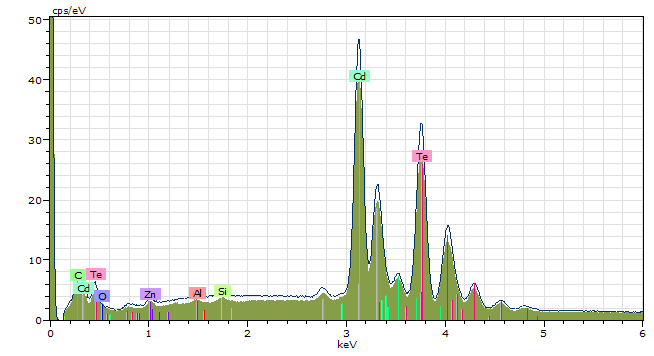
\includegraphics[width=\linewidth]{subB2b_sem_03_m002_eds.png}
          \end{minipage}
          \begin{minipage}[c]{0.11\linewidth}
            \centering
            \atomicTable[\ce{Cd}&\SI{44.8}{}][\ce{Te}&\SI{44.6}{}][\ce{Zn}&\SI{1.9}{}][\ce{C}&\SI{6.4}{}][\ce{O}&\SI{1.1}{}][\ce{Al}&\SI{0.7}{}][\ce{Si}&\SI{0.5}{}]%OK
          \end{minipage}
    \end{subfigure}
    \par\bigskip
    \begin{subfigure}[t]{\textwidth}
        \caption{}\label{fig:subB2b_C2F5}
          \begin{minipage}[c]{0.43\linewidth}
            \centering
            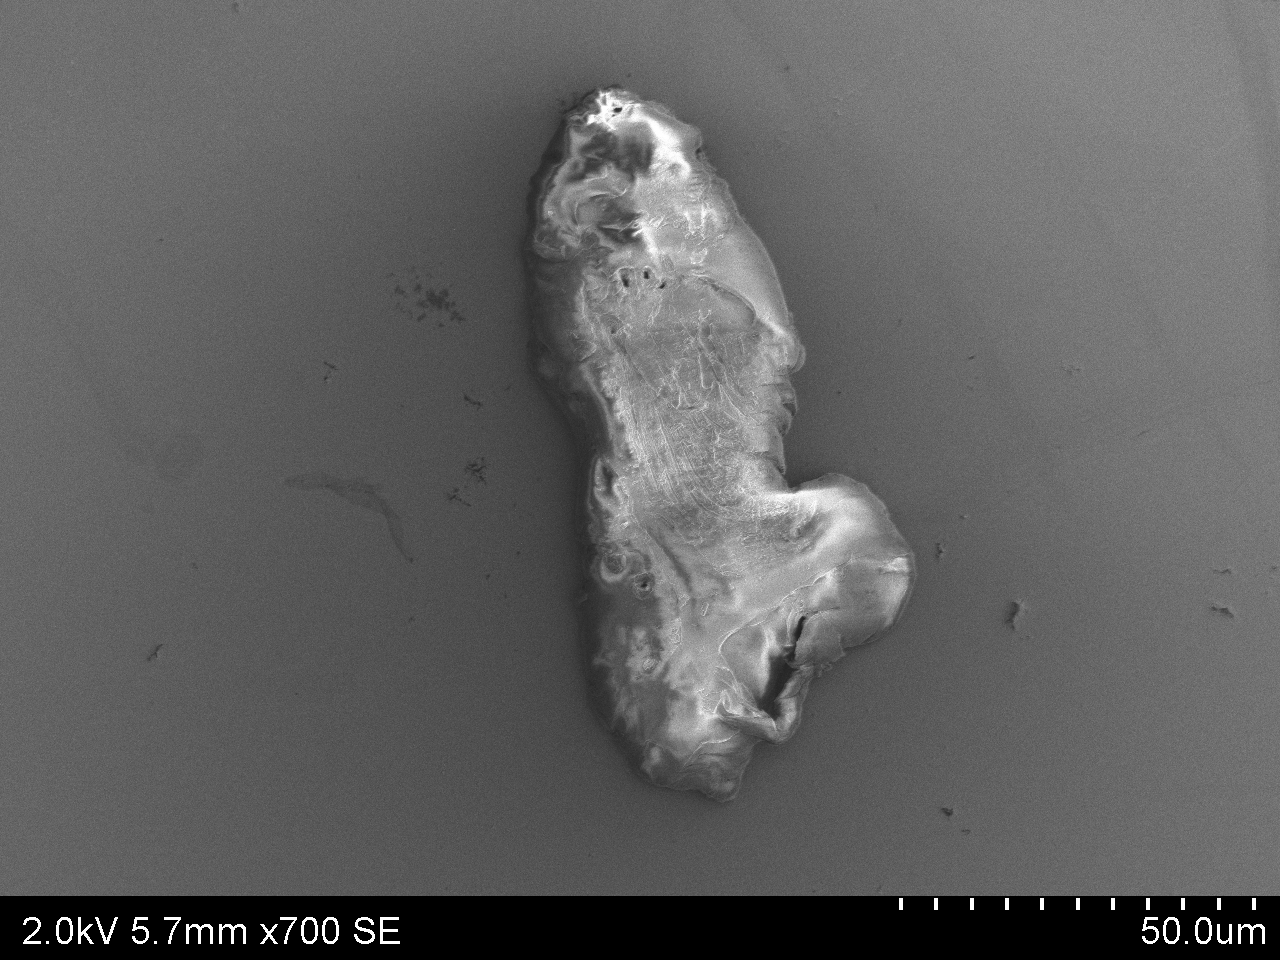
\includegraphics[width=\linewidth]{subB2b_sem_03_m001.png}
          \end{minipage}
          \hfill
          \begin{minipage}[c]{0.43\linewidth}
            \centering
            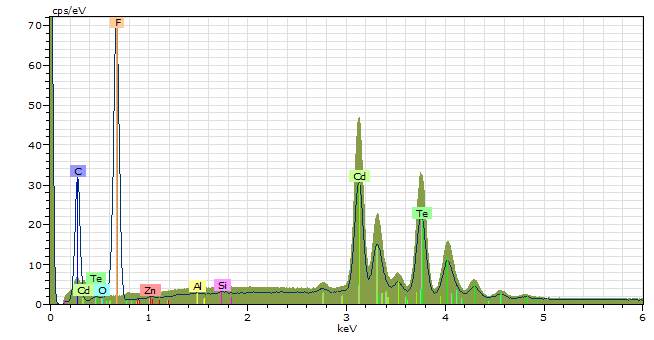
\includegraphics[width=\linewidth]{subB2b_sem_03_m001_eds.png}
          \end{minipage}
          \begin{minipage}[c]{0.11\linewidth}
            \centering
            \atomicTable[\ce{F}&\SI{55.8}{}][\ce{C}&\SI{22.5}{}][\ce{Cd}&\SI{10.6}{}][\ce{Te}&\SI{10.4}{}][\ce{O}&\SI{0.4}{}][\ce{Zn}&\SI{0.2}{}][\ce{Si}&\SI{0.1}{}] %[\ce{}&\SI{}{}]%OK
          \end{minipage}
    \end{subfigure}
    \caption[\Ac{sem} images, \ac{eds} spectra, and \ac{eds} atomic compositions of four different types of particles found on substrate B and substrate B2 after surface pre-growth preparation.]{High resolution \ac{sem} images of four different types of particles found on substrate B and substrate B2 after surface pre-growth preparation and the corresponding \ac{eds} spectra and atomic compositions: \subref{fig:subB2b_alumina} Alumina (\ce{Al2O3}) polishing grit agglomeration; \subref{fig:subB2b_czt} cadmium zinc telluride (\ce{Cd_{0.96}Zn_{0.04}Te}) particle.; \subref{fig:subB2b_C2F5} particle based on flouride (\ce{F}) and carbon (\ce{C}); and \subref{fig:subB2b_mct} mercury telluride (\ce{HgTe}) particle. The blue spectra represent the particle and the green spectra represent the surrounding substrate.}\label{fig:subBb_sem_w_eds}
\end{figure}
%
\begin{figure}[htbp]
\ContinuedFloat
    \centering
    \begin{subfigure}[t]{\textwidth}
        \caption{}\label{fig:subB2b_mct}
          \begin{minipage}[c]{0.43\linewidth}
            \centering
            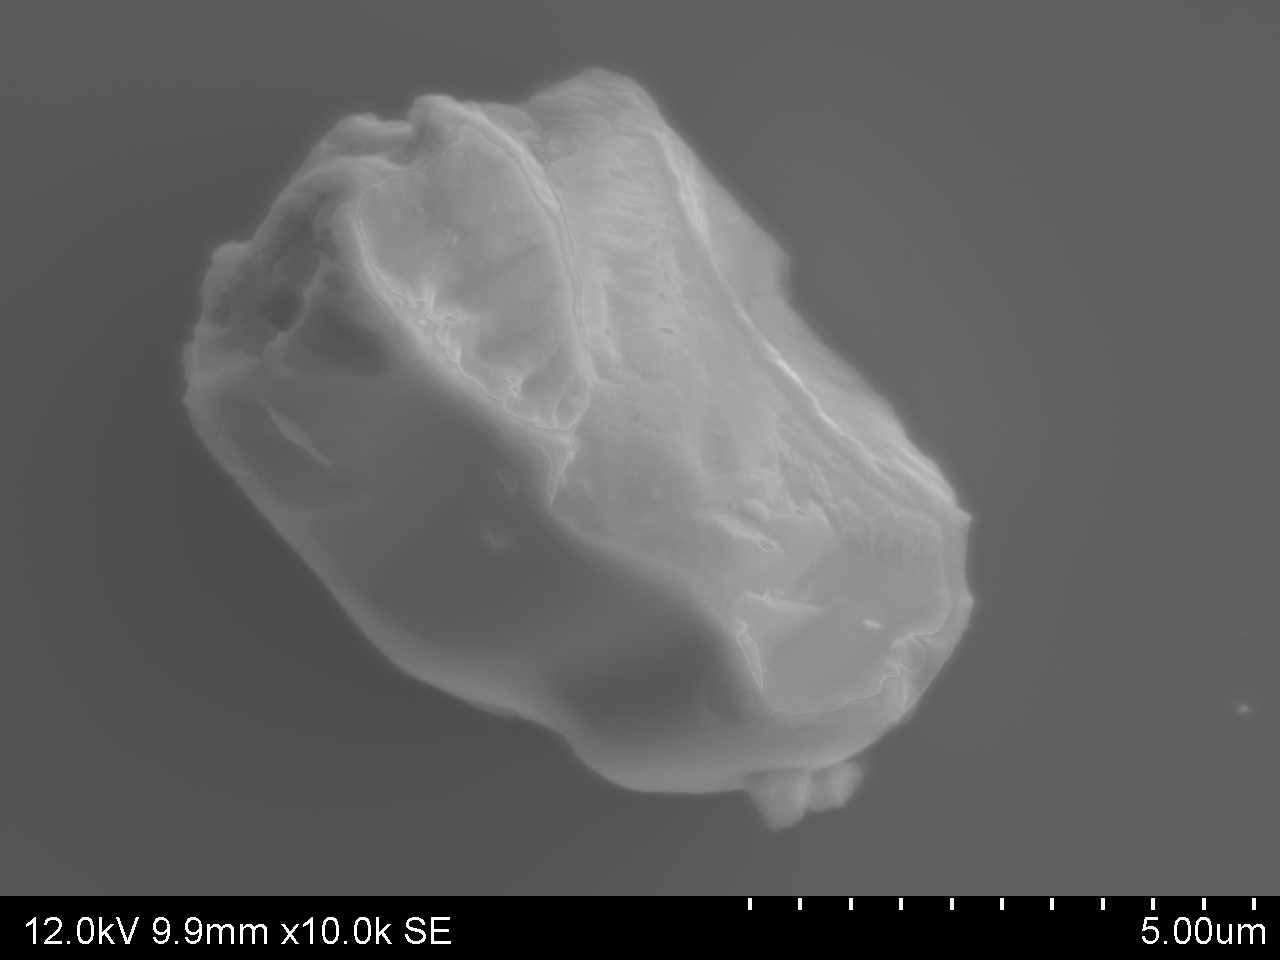
\includegraphics[width=\linewidth]{subB2b_sem_04_m010.png}
          \end{minipage}
          \hfill
          \begin{minipage}[c]{0.43\linewidth}
            \centering
            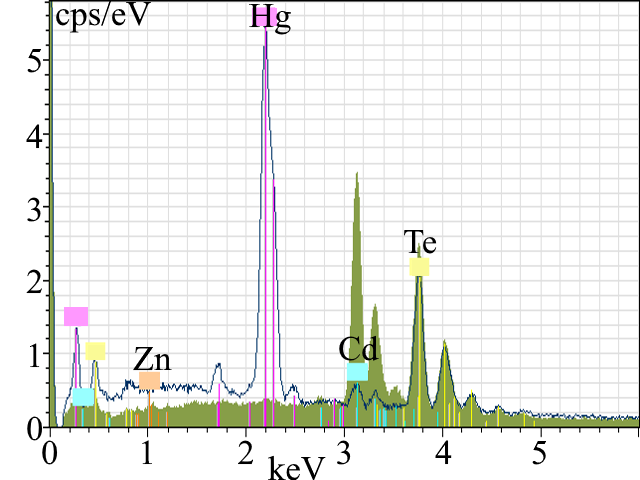
\includegraphics[width=\linewidth]{subB2b_sem_04_m010_eds.png}
          \end{minipage}
          \begin{minipage}[c]{0.11\linewidth}
            \centering
            \atomicTable[\ce{Te}&\SI{35.7}{}][\ce{Hg}&\SI{31.0}{}][\ce{C}&\SI{30.4}{}][\ce{Cd}&\SI{2.81}{}][\ce{Zn}&\SI{0.1}{}]%OK
          \end{minipage}
    \end{subfigure}
    \captionsetup{list=no}
    \caption{\emph{(continued)}}
\end{figure}

\subsubsection{Alumina (\ce{Al2O3}) polishing grit}

The small particles observed in \ac{sem} were distributed over the surface with a tendency of higher density towards the upper right, lower right, and lower left corners. The particle density on substrate B was found to be between \SI{2e+06}{\centi\metre^{-2}} and \SI{2e+07}{\centi\metre^{-2}}. The average particle density was \SI{7e+06}{\centi\metre^{-2}} with a standard deviation of \SI{4e+06}{\centi\metre^{-2}}. A graphical representation of the particle density at different locations on substrate B can be seen in Fig.~\ref{fig:subBb_densityData}.

Substrate B2 had a similar distribution of polishing grit. There were higher densities of particles near the left and upper edges. The particle density was found to be between \SI{2e+06}{\centi\metre^{-2}} and \SI{6e+07}{\centi\metre^{-2}}. The average particle density was \SI{1e+07}{\centi\metre^{-2}} with a standard deviation of \SI{1e+07}{\centi\metre^{-2}}. A graphical representation of the particle density at different locations on substrate B2 can be seen in Fig.~\ref{fig:subB2b_densityData}.

\begin{figure}[htbp]
    \centering
    \mySubfigure{0.49\textwidth}{subBb_densityData.png}[fig:subBb_densityData]
    \hfill
    \mySubfigure{0.49\textwidth}{subB2b_densityData.png}[fig:subB2b_densityData]
    \caption[Maps of the polishing grit density on substrates B and B2 after surface pre-growth preparation.]{Maps of the polishing grit density on the $\SI{30}{\milli\metre}\times\SI{30}{\milli\metre}$ substrates B and B2 after surface pre-growth preparation: \subref{fig:subBb_densityData} 36 different locations on substrate B where the polishing grit density varied between \SI{2e+06}{\centi\metre^{-2}} and \SI{2e+07}{\centi\metre^{-2}}; and \subref{fig:subB2b_densityData} 36 different locations on substrate B2 where the polishing grit density varied between \SI{2e+06}{\centi\metre^{-2}} and \SI{6e+07}{\centi\metre^{-2}}. The density measurements were obtained by counting the number of polishing grits in \ac{sem} images covering $\SI{25.4}{\micro\metre}\times\SI{17.8}{\micro\metre}$ areas. In total, \SI{0.002}{\percent} of the substrate surfaces were measured.}
    \label{fig:subBb_and_subB2b_densityData}
\end{figure}

\subsubsection{\ce{Cd_{0.96}Zn_{0.04}Te} particles}
\todo{}

\subsubsection{Particle composed of flouride and carbon}
\todo{Diskuter hvor denne kommer fra.}

\subsubsection{\ce{HgTe} particles}
\todo{}

\begin{comment}
\todo{Fiks dette et sted.}
In order to observe correlations between the occurrence of voids and microvoids on the as-received substrate B to the occurrence of polishing grit after polish and etch, the sample Pearson correlation coefficient was determined. \todo{Skriv inn formel. Og regn ut correlation.} If there are one dataset $x_i \in \{x_1, ..., x_n\}$ containing $n$ values and another dataset $y_i \in \{y_1, ..., y_n\}$ containing $n$ values, then the sample Pearson correlation coefficient is defined as

\begin{equation}\label{eq:pearson_correlation_coefficient}
    r = \frac{
        n\sum_{i=1}^nx_iy_i - \sum_{i=1}^n x_i \sum_{i=1}^n y_i
        }{
        \sqrt{n\sum_{i=1}^n x_i^2 - \parentheses{\sum_{i=1}^n x_i}^2}\sqrt{n\sum_{i=1}^n y_i^2 - \parentheses{\sum_{i=1}^n y_i}^2} },
\end{equation}
where $\avg{x}=\frac{1}{n}\sum_{i=1}^n x_i$ is the sample mean; and analogously for $\avg{y}$. 

%Correlation is an effect size and so we can verbally describe the strength of the correlation using the guide that Evans (1996) suggests for the absolute value of r. .00-.19 “very weak” .20-.39 “weak” .40-.59 “moderate” .60-.79 “strong” .80-1.0 “very strong”
%
%\begin{equation}
%    r = \frac{\sum_{i=1}^n x_i y_i - n\avg{x}\avg{y}}{\parentheses{n-1}s_xs_y},
%\end{equation}
%where $s_x = \sqrt{\frac{1}{n-1}\sum_{i=1}^n \parentheses{x_i - \avg{x}}^2}$ is the sample standard deviation; and analogously for $s_y$.
\end{comment}

%%=========================================
%\section{AFM Study of Polished and Etched Substrate B}
\subsection{Surface Roughness}
\todo{Fig.~\ref{fig:subBb_and_subB2_afm} or Fig~\ref{fig:subBb_afm_centre}--\oldsubref{fig:subBb_afm_corner} substrate B; and Fig.~\ref{fig:subB2b_afm_centre}--\oldsubref{fig:subB2b_afm_corner} substrate B2.}

\begin{figure}[htbp]
    \centering
    \begin{subfigure}[c]{0.032\linewidth}
        \label{fig:subBb_afm_scale}\captionsetup{list=no}
        
\includegraphics[width=\linewidth]{subBb_afm_scale.png}
    \end{subfigure}
    \hfill
    \mySubfigure{0.3\linewidth}{subBb_afm_centre.png}[fig:subBb_afm_centre]%\SI{0.85}{\nano\metre}
    \hfill
    \mySubfigure{0.3\linewidth}{subBb_afm_leftedge.png}[fig:subBb_afm_edge]%\SI{0.77}{\nano\metre}
    \hfill
    \mySubfigure{0.3\linewidth}{subBb_afm_upperleftcorner.png}[fig:subBb_afm_corner] %\SI{1,04}{\nano\metre}}
    \par\bigskip
    \begin{subfigure}[c]{0.032\linewidth}
        \label{fig:subB2b_afm_scale}\captionsetup{list=no}
        
\includegraphics[width=\linewidth]{subB2b_afm_scale.png}
    \end{subfigure}
    \hfill
    \mySubfigure{0.3\linewidth}{subB2b_afm_centre.png}[fig:subB2b_afm_centre]
    \hfill
    \mySubfigure{0.3\linewidth}{subB2b_afm_upperedge.png}[fig:subB2b_afm_edge]
    \hfill
    \mySubfigure{0.3\linewidth}{subB2b_afm_upperleftcorner.png}[fig:subB2b_afm_corner]
    \caption[\Ac{afm} of substrate B and substrate B2 with surface pre-growth preparation.]{\Ac{afm} measurements of substrate B and substrate B2 with surface pre-growth preparation. Images of $\SI{5}{\micro\metre}\times\SI{5}{\micro\metre}$ areas are taken at three different locations on the substrate surfaces. For substrate B: \subref{fig:subBb_afm_centre} near the centre, \ac{rms} roughness \SI{0.85}{\nano\metre}; \subref{fig:subBb_afm_edge} near the left edge, \ac{rms} roughness \SI{0.76}{\nano\metre}; and \subref{fig:subBb_afm_corner} near the upper left corner, \ac{rms} roughness \SI{0.92}{\nano\metre}. For substrate B2: \subref{fig:subB2b_afm_centre} near the centre, \ac{rms} roughness \SI{0.91}{\nano\metre}; \subref{fig:subB2b_afm_edge} near the upper edge, \ac{rms} roughness \SI{0.96}{\nano\metre}; and \subref{fig:subB2b_afm_corner} near the upper left corner, \ac{rms} roughness \SI{1.3}{\nano\metre}.}\label{fig:subBb_and_subB2_afm}
\end{figure} % AFM, substrate B, with surface pre-growth preparation.

% B2: AFM: UL - 1.310 nm, U-edge - 0.956, Centre- 0.912 nm

%%=========================================
\subsection{Impurity Analysis -- EDS}

\todo{Sammenlign med før. Sett inn for B/B2.}

\begin{table}[htbp]
    \centering
    \caption[\Ac{eds} impurity analysis of substrate B with surface pre-growth preparation.]{Results of the \ac{eds} impurity analysis at three different locations on the $\SI{30}{\milli\metre}\times\SI{30}{\milli\metre}$ (111)B \ac{czt} substrate B with surface pre-growth preparation (atomic concentration \%). The X-ray signal is acquired from $\SI{1270}{\micro\metre}\times\SI{890}{\micro\metre}$ areas near the centre, upper edge, and upper left corner.}\label{tab:subBb_eds_analysis}
    \begin{tabu} to 1.0\textwidth { X[1.85,r] X[1.125,c] X[1.125,c] X[1.125,c] X[1.125,c] X[1.125,c] X[1.125,c] X[1.125,c] }
    \hline
         & \textbf{\ce{Te}} (at.\%) & \textbf{\ce{Cd}} (at.\%) & \textbf{\ce{Zn}} (at.\%) & \textbf{\ce{Al} } (at.\%) & \textbf{\ce{Si}} (at.\%) & \textbf{\ce{C}} (at.\%) & \textbf{\ce{O}} (at.\%) \\
        \hline
        Near centre  & \SI{46.10}{} & \SI{45.35}{} & \SI{1.92}{} & \SI{0.23}{} & \SI{0.52}{} & \SI{5.49}{} & \SI{0.40}{} \\ % \SI{15.0}{} & \SI{15.0}{}
        Near edge & \SI{45.49}{} & \SI{45.12}{} & \SI{2.02}{} & \SI{0.26}{} & \SI{0.49}{} & \SI{5.99}{} & \SI{0.64}{} \\ % \SI{15.0}{} & \SI{29.0}{}
        Near corner & \SI{45.83}{} & \SI{45.34}{} & \SI{1.92}{} & \SI{0.60}{} & \SI{0.50}{} & \SI{5.34}{} & \SI{0.47}{} \\ % \SI{1.0}{}  & \SI{29.0}{}
         \hline
    \end{tabu}
\end{table}
%%=========================================
% FTIR transmission spectra.
%\subsection{IR Characterisation}

%\todo{Have our preparation method --> domene O fletter som vi bare ser i IR-gjennomlysing. Kommenter.}

%%=========================================
